\documentclass[10pt,a4paper]{article}

\usepackage[a4paper,margin=1.55cm,top=1.45cm,bottom=1.45cm]{geometry}
\usepackage[T1]{fontenc}
\usepackage{newtxtext,newtxmath}
\usepackage{microtype}
\usepackage{graphicx}
\usepackage{booktabs}
\usepackage{tabularx}
\usepackage{amsmath}
\usepackage{xcolor}
\usepackage{caption}
\usepackage{enumitem}
\usepackage[round,authoryear]{natbib}
\usepackage{titlesec}
\usepackage{fancyhdr}
\usepackage[hidelinks]{hyperref}

\definecolor{accent}{HTML}{1F5C5A}
\hypersetup{
  colorlinks=true,
  linkcolor=accent,
  citecolor=accent,
  urlcolor=accent,
  pdftitle={Beyond Gender-Only Fairness: Extending FairTrade to Gender and Race},
  pdfauthor={Rony Souz}
}
\urlstyle{same}
\setlength{\parindent}{0pt}
\setlength{\parskip}{3.2pt}
\setlength{\bibsep}{2.5pt}
\setlist{nosep,leftmargin=1.4em}
\captionsetup{font=small,labelfont=bf,skip=3pt,hypcap=false}
\titleformat{\section}{\large\bfseries\color{accent}}{}{0pt}{}
\titlespacing*{\section}{0pt}{7pt}{3pt}
\titleformat{\subsection}{\normalsize\bfseries}{}{0pt}{}
\titlespacing*{\subsection}{0pt}{5pt}{2pt}
\pagestyle{fancy}
\fancyhf{}
\renewcommand{\headrulewidth}{0pt}
\fancyfoot[C]{\small\thepage}
\setlength{\footskip}{0.65cm}
\newcommand{\ppr}{\operatorname{PPR}}
\newcommand{\tasktag}[1]{\textcolor{accent}{\textbf{Task #1}}}

\begin{document}

{\fontsize{18}{21}\selectfont\bfseries Beyond Gender-Only Fairness:\\[-1pt]
Extending FairTrade to Gender and Race}\par
\vspace{3pt}
{\large HiWi Coding Challenge Report}\hfill{\normalsize\textbf{Rony Souz}}\par
\vspace{2pt}
\small 15 July 2026 \quad\textbullet\quad
\href{https://github.com/Ronyszx/HiWi_FairTrade}{github.com/Ronyszx/HiWi\_FairTrade}
\quad\textbullet\quad branch: \texttt{rony-challenge-work}
\vspace{4pt}
\hrule
\vspace{4pt}

FairTrade studies the trade-off between balanced accuracy and fairness in federated learning through multi-objective Bayesian optimization (MOBO) \citep{badar2024fairtrade,badarFairTradeCode}. The original Adult experiment treats gender as its sensitive attribute. I followed the challenge from reproduction, through a race and intersectional audit, to a joint gender--race extension. I also studied FAC-Fed because it places a fairness intervention in client-local processing before aggregation \citep{badar2023facfed,badarFacFedCode}. I did not copy its method: FAC-Fed addresses adaptive augmentation, streaming and non-IID data, and concept drift, rather than this two-attribute MOBO problem.

\section*{Reproducing FairTrade \hfill \tasktag{1}}

I first ran the Adult baseline with three clients, statistical parity, 15 local epochs, 50 communication rounds, 10 MOBO iterations per round, random client distribution, seed 42, and CPU execution. The final model reached a balanced accuracy of \textbf{0.7690318211867191} and signed statistical parity difference (SPD) of \textbf{0.02843397520847807}. The accuracy is close to the FairTrade Adult value around 0.77, while my SPD is materially above the comparable reported value near 0.001. I therefore treat this as a successful baseline execution, not an exact numerical reproduction.

In the repository, the fairness weight $\alpha$ and learning rate are MOBO inputs. Balanced accuracy and fairness are competing outputs. qEHVI proposes candidates expected to expand the dominated hypervolume. A point is Pareto-optimal when one objective cannot be improved without worsening another. After candidate evaluation, the code uses a weighted sum over the Pareto set to choose the next round's hyperparameters. The saved histories contain one evaluation at the \emph{start} of each communication round; they are not the final-model values printed after all training and candidate evaluations.

For portability, I added an explicit seed and validated device selection without altering the fixed dataset split. I also made result-directory creation automatic. These changes made repeated CPU smoke tests identical while keeping the baseline protocol readable and easy to reproduce.

\vfill
\newpage

\section*{What Gender-Only Evaluation Missed \hfill \tasktag{2}}

I evaluated the final baseline predictions on the 6,513-row Adult test split \citep{becker1996adult}. For a group $A$, $\ppr(A)=P(\hat{Y}=1\mid A)$. I used the repository's direction conventions
\[
 \mathrm{SPD}_{g}=\ppr(\mathrm{Male})-\ppr(\mathrm{Female}),\qquad
 \mathrm{SPD}_{r}=\ppr(\mathrm{White})-\ppr(\mathrm{NonWhite}).
\]
The intersectional groups were White Male, White Female, Non-White Male, and Non-White Female. Their max--min gap is $\max_k\ppr(k)-\min_k\ppr(k)$.

\begin{center}
\small
\begin{tabular}{lrr@{\hspace{1.0cm}}lrr}
\toprule
Group & $n$ & PPR & Group & $n$ & PPR \\
\midrule
Male & 4,360 & 0.4733944954 & Female & 2,153 & 0.4449605202 \\
White & 5,568 & 0.4908405172 & Non-White & 945 & 0.3058201058 \\
White Male & 3,836 & 0.4960896767 & White Female & 1,732 & 0.4792147806 \\
Non-White Male & 524 & 0.3072519084 & Non-White Female & 421 & 0.3040380048 \\
\bottomrule
\end{tabular}
\end{center}

The absolute gender SPD was only \textbf{0.0284339752}. In isolation, that result looked reasonably small. Race told a different story: the absolute race SPD was \textbf{0.1850204114}, and the intersectional max--min gap was \textbf{0.1920516720}. The White Male group had the highest positive prediction rate and the Non-White Female group the lowest.

\begin{center}
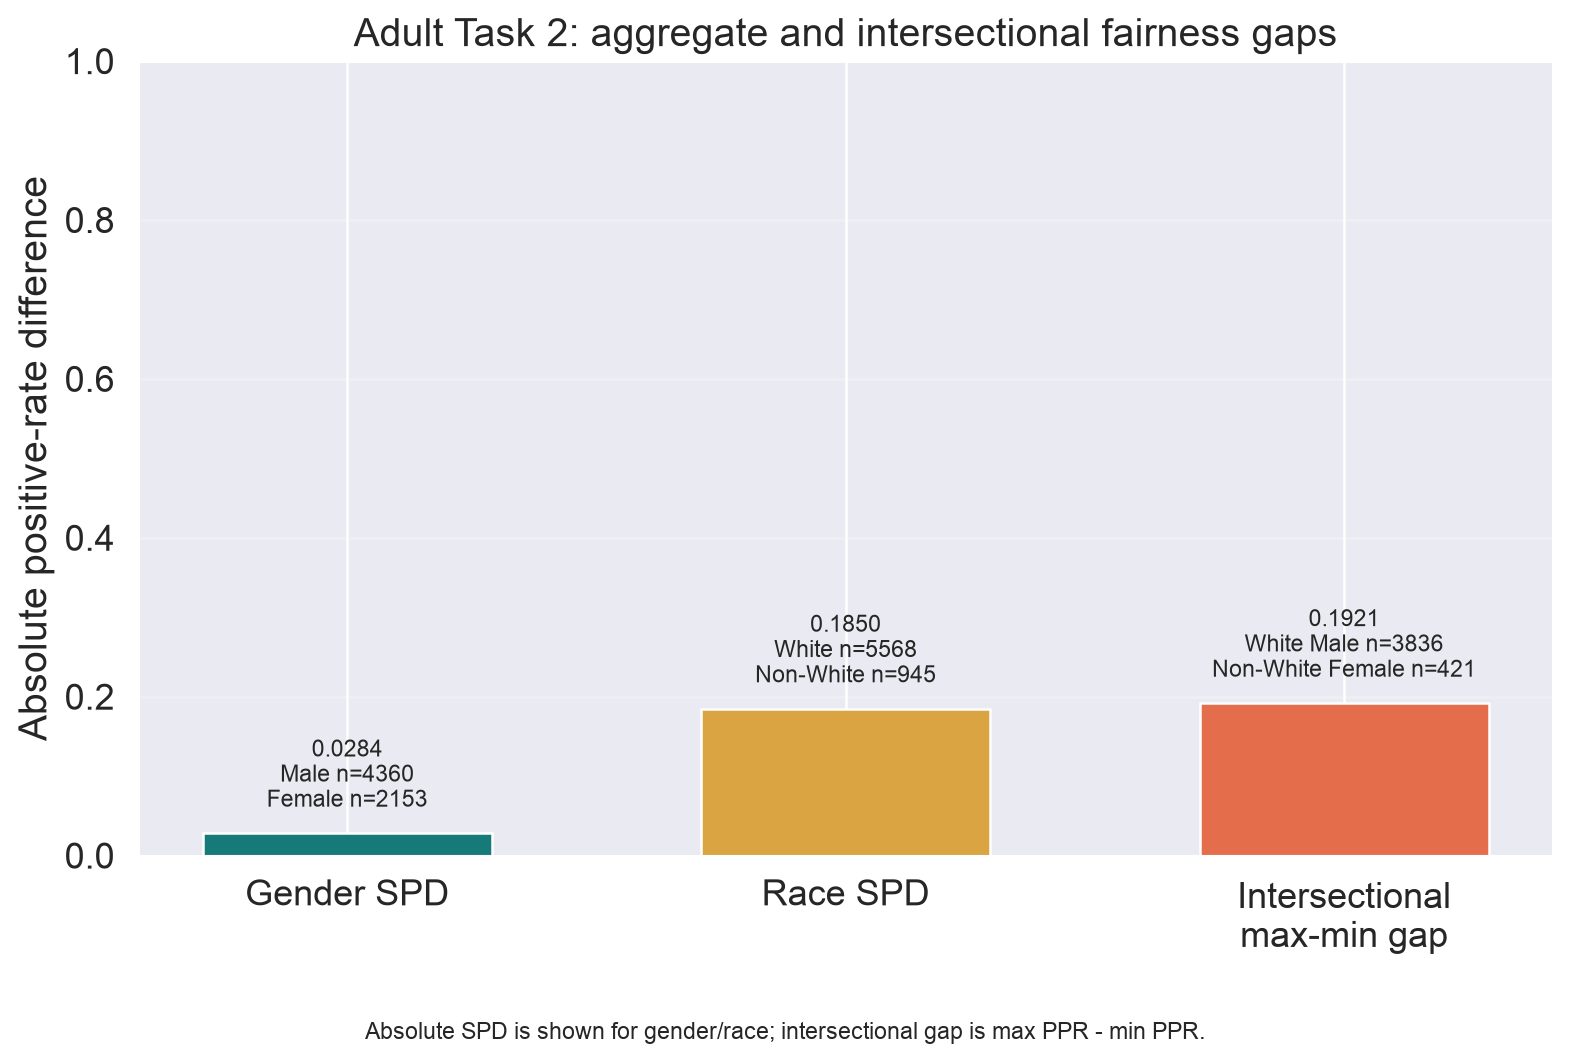
\includegraphics[width=0.75\linewidth]{figures/task2_intersectional_spd.png}
\captionof{figure}{The gender-only gap is small relative to the race and intersectional gaps. Counts in the chart also show that the four groups are unevenly represented.}
\end{center}

This is the practical concern behind fairness gerrymandering: acceptable aggregate fairness need not imply comparable outcomes for meaningful subgroups \citep{kearns2018gerrymandering}. It motivated me to include race in training rather than only adding another metric after training. The audit still has a limitation: collapsing every non-White race category into one binary group can hide disparities within that combined group.

\vfill
\newpage

\section*{Optimizing Gender and Race Together \hfill \tasktag{3}}

\subsection*{Local objective}
I kept FairTrade's structure and changed only the opt-in Task 3 fairness path. Each client used
\[
 \mathcal{L}_{\mathrm{fair}}=0.5\,\mathcal{L}_{\mathrm{DP,gender}}
                              +0.5\,\mathcal{L}_{\mathrm{DP,race}}.
\]
Both attributes therefore contribute gradients. Equal averaging also keeps the fairness-loss scale close to the original single-attribute loss. I preferred this smooth combination to a hard maximum, which could switch abruptly between attributes during gradient training. These local demographic-parity losses use continuous model outputs; they are differentiable surrogates and are not numerically identical to SPD computed from rounded final predictions.

\subsection*{MOBO objective}
For candidate evaluation I computed signed $\mathrm{SPD}_{g}$ and $\mathrm{SPD}_{r}$ from aligned predictions and sensitive attributes, then defined
\[
 V_{\mathrm{worst}}=\max\!\left(|\mathrm{SPD}_{g}|,|\mathrm{SPD}_{r}|\right),
 \qquad \mathbf{f}=\left[-V_{\mathrm{worst}},\;\mathrm{balanced\ accuracy}\right].
\]
An average could hide one large disparity behind one small disparity. The maximum instead exposes the currently worse attribute while preserving FairTrade's two-objective design. This was simpler to interpret than introducing a three-objective optimizer. Since $-V_{\mathrm{worst}}\in[-1,0]$ and balanced accuracy is non-negative, I used the qEHVI reference point $[-1.01,-0.01]$, which is dominated by feasible outcomes.

\subsection*{Final result}
The final balanced accuracy was \textbf{0.7683912709437309}. Signed and absolute gender SPD were \textbf{0.010463530725209502}; signed and absolute race SPD were \textbf{0.0003118728334245424}. Thus the worst absolute SPD was \textbf{0.010463530725209502}. The intersectional max--min gap was \textbf{0.09037460789468915}.

\begin{center}
\small
\begin{tabularx}{\linewidth}{@{}Xrrr@{}}
\toprule
Metric & Task 1 & Task 3 & Relative reduction \\
\midrule
Balanced accuracy & 0.7690 & 0.7684 & n/a \\
Absolute gender SPD & 0.0284 & 0.0105 & 63.2\% \\
Absolute race SPD & 0.1850 & 0.0003 & 99.8\% \\
Worst absolute SPD & 0.1850 & 0.0105 & 94.3\% \\
Intersectional max--min gap & 0.1921 & 0.0904 & 52.9\% \\
\bottomrule
\end{tabularx}
\end{center}

Balanced accuracy decreased by \textbf{0.0006405502} in absolute terms; this is an accuracy change, not a fairness reduction. The large relative reductions above describe lower disparity, not percentage-point changes.

\begin{center}
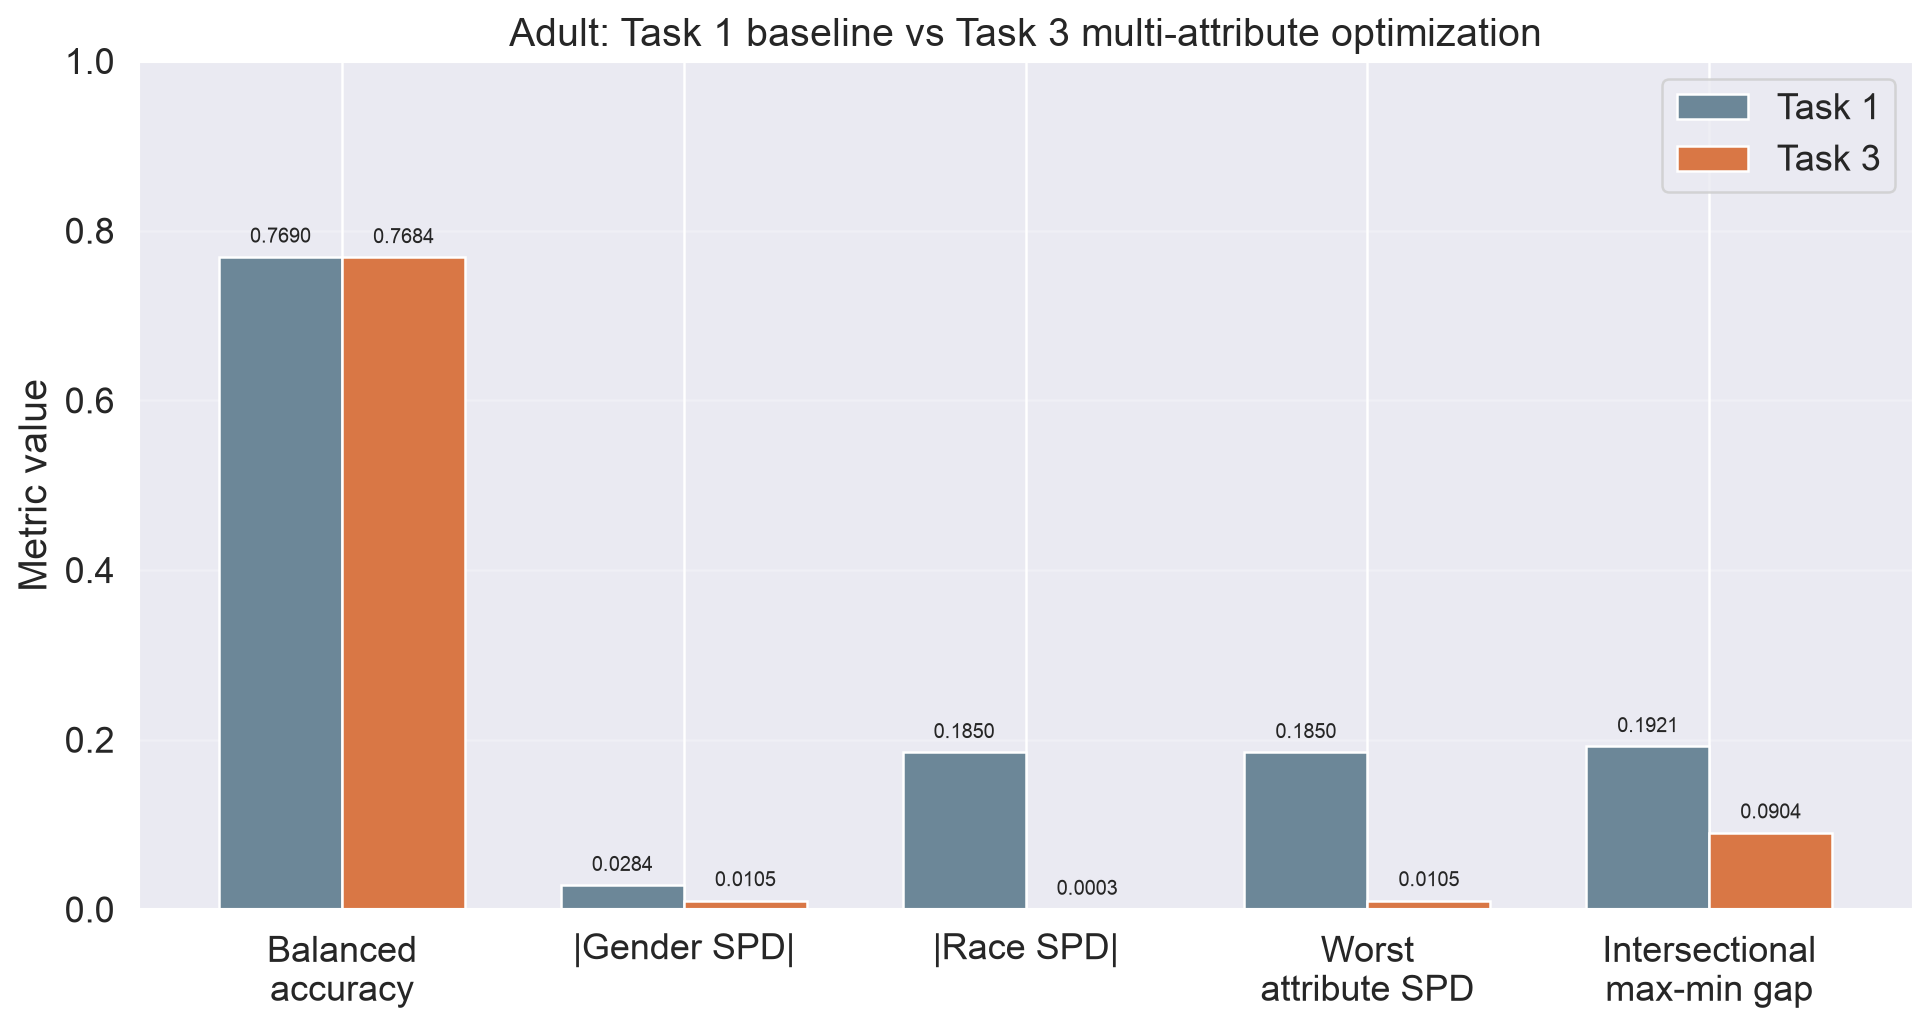
\includegraphics[width=0.90\linewidth]{figures/task1_vs_task3.png}
\captionof{figure}{Task 3 nearly preserves balanced accuracy while reducing both marginal SPDs and the worst marginal disparity. The remaining intersectional gap is still visible.}
\end{center}

\newpage
\subsection*{Interpretation and recovery}
Marginal gender and race fairness improved substantially, and race SPD became nearly zero rather than exactly zero. However, an intersectional gap near 0.0904 remained. Optimizing the two attributes marginally did not guarantee equal outcomes across all four intersections. One GP fit failed at communication round 13, MOBO iteration 10. The Task 3-only recovery retained the previous valid $\alpha$ and learning rate, skipped the remaining search in that round, appended no failed observation, and completed all 50 rounds.

\section*{Code Review and Bug Hunt \hfill \tasktag{4}}

The formal bug I found was a return-value mismatch in the first optimization-loop call. It attempted
\begin{center}
\texttt{objectives, bal\_acc\_, fairness\_notion\_ = evaluate(alpha)}
\end{center}
although \texttt{evaluate()} returns one object: the two-column \texttt{objectives} tensor. Training and the first evaluation completed, but Python then raised \texttt{ValueError} with ``not enough values to unpack,'' so MOBO could not continue. The minimal repair assigned the returned tensor directly:
\begin{center}
\texttt{objectives = evaluate(alpha)}
\end{center}
Later code already reads fairness and balanced accuracy from the tensor columns, so extra return values were unnecessary.

\section*{Limitations}

The original model ends with a Sigmoid, local training uses \texttt{BCEWithLogitsLoss}, and \texttt{ConstraintLoss} applies another sigmoid. The first three baseline behaviors I preserved for comparability were this existing loss pipeline, MOBO use of the test split, and the nested loop's repeated candidate evaluation. They remain methodological concerns rather than hidden fixes. Race was reduced to White versus Non-White, only one seed and the requested Adult configuration received a full run, and Task 3 did not eliminate intersectional disparity.

\section*{Conclusion}

Reproduction established balanced accuracy near 0.77. The subgroup audit then showed that a modest gender gap concealed a much larger race-associated gap. Joint optimization reduced the worst marginal disparity with only a small accuracy decrease, but the residual intersectional gap matters. My result therefore improves marginal treatment across gender and race while showing why intersectional fairness remains a separate, harder objective.

\clearpage
\begingroup
\footnotesize
\bibliographystyle{plainnat}
\bibliography{references}
\endgroup

\end{document}
